\documentclass{article}
\usepackage{tikz}
\usetikzlibrary{arrows.meta}

\begin{document}

\begin{figure}[h]
    \centering
    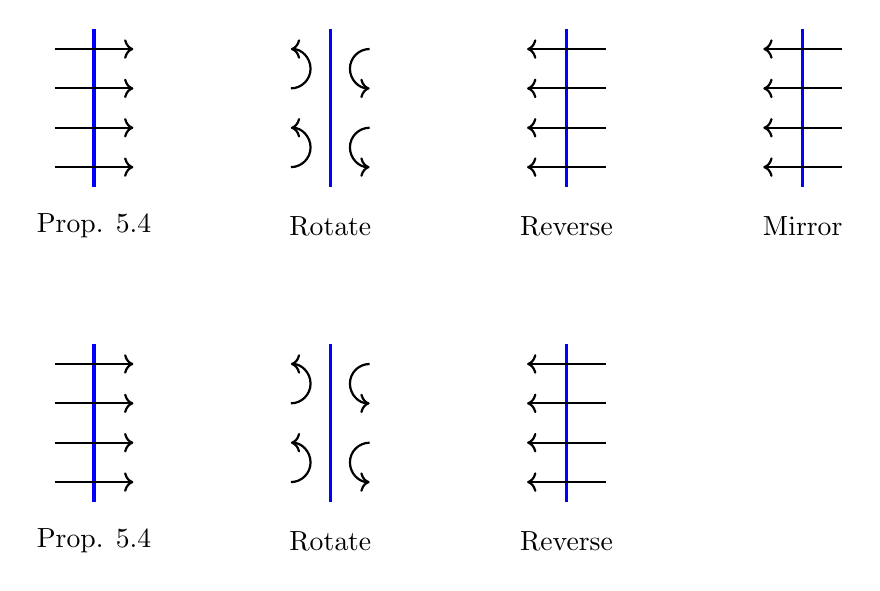
\begin{tikzpicture}[scale=0.5]
        % Original configuration (Prop. 5.4)
        \draw[blue, very thick] (0,0) -- (0,4);
        \draw[->, thick] (-1,0.5) -- (1,0.5);
        \draw[->, thick] (-1,1.5) -- (1,1.5);
        \draw[->, thick] (-1,2.5) -- (1,2.5);
        \draw[->, thick] (-1,3.5) -- (1,3.5);
        \node at (0,-1) {Prop. 5.4};
        
        % Rotated configuration
        \begin{scope}[xshift=6cm]
            \draw[blue, very thick] (0,0) -- (0,4);
            \draw[->, thick] (-1,0.5) arc (-90:90:0.5);
            \draw[->, thick] (1,1.5) arc (90:270:0.5);
            \draw[->, thick] (-1,2.5) arc (-90:90:0.5);
            \draw[->, thick] (1,3.5) arc (90:270:0.5);
            \node at (0,-1) {Rotate};
        \end{scope}
        
        % Reversed configuration
        \begin{scope}[xshift=12cm]
            \draw[blue, very thick] (0,0) -- (0,4);
            \draw[->, thick] (1,0.5) -- (-1,0.5);
            \draw[->, thick] (1,1.5) -- (-1,1.5);
            \draw[->, thick] (1,2.5) -- (-1,2.5);
            \draw[->, thick] (1,3.5) -- (-1,3.5);
            \node at (0,-1) {Reverse};
        \end{scope}
        
        % Mirror image (horizontal reflection) of original
        \begin{scope}[xshift=18cm]
            \draw[blue, very thick] (0,0) -- (0,4);
            \draw[->, thick] (1,0.5) -- (-1,0.5);
            \draw[->, thick] (1,1.5) -- (-1,1.5);
            \draw[->, thick] (1,2.5) -- (-1,2.5);
            \draw[->, thick] (1,3.5) -- (-1,3.5);
            % Note: This is effectively the same as the "Reverse" step above, 
            % but labeled as a mirror image.
            \node at (0,-1) {Mirror};
        \end{scope}
        
        % Repeat for the lower row as the same as above but shifted down
        \begin{scope}[yshift=-8cm]
            % Original configuration (Prop. 5.4)
            \draw[blue, very thick] (0,0) -- (0,4);
            \draw[->, thick] (-1,0.5) -- (1,0.5);
            \draw[->, thick] (-1,1.5) -- (1,1.5);
            \draw[->, thick] (-1,2.5) -- (1,2.5);
            \draw[->, thick] (-1,3.5) -- (1,3.5);
            \node at (0,-1) {Prop. 5.4};
            
            % Rotated configuration
            \begin{scope}[xshift=6cm]
                \draw[blue, very thick] (0,0) -- (0,4);
                \draw[->, thick] (-1,0.5) arc (-90:90:0.5);
                \draw[->, thick] (1,1.5) arc (90:270:0.5);
                \draw[->, thick] (-1,2.5) arc (-90:90:0.5);
                \draw[->, thick] (1,3.5) arc (90:270:0.5);
                \node at (0,-1) {Rotate};
            \end{scope}
            
            % Reversed configuration
            \begin{scope}[xshift=12cm]
                \draw[blue, very thick] (0,0) -- (0,4);
                \draw[->, thick] (1,0.5) -- (-1,0.5);
                \draw[->, thick] (1,1.5) -- (-1,1.5);
                \draw[->, thick] (1,2.5) -- (-1,2.5);
                \draw[->, thick] (1,3.5) -- (-1,3.5);
                \node at (0,-1) {Reverse};
            \end{scope}
        \end{scope}
    \end{tikzpicture}
    \caption{The saddle moves of Proposition \ref{prop:newii} are consistent under mirror image, as explained in the proof of Proposition \ref{prop:newimirror}.}
\end{figure}

\end{document}